\documentclass[12pt]{article}
\usepackage{tikz}
\usepackage{pgfplots}
\pgfplotsset{compat=1.13}

\usepackage{extsizes}
\usepackage{caption}
\usepackage{multirow}

\renewcommand{\epsilon}{\ensuremath{\varepsilon}}
\renewcommand{\phi}{\ensuremath{\varphi}}
\renewcommand{\kappa}{\ensuremath{\varkappa}}
\renewcommand{\le}{\ensuremath{\leqslant}}
\renewcommand{\leq}{\ensuremath{\leqslant}}
\renewcommand{\ge}{\ensuremath{\geqslant}}
\renewcommand{\geq}{\ensuremath{\geqslant}}
\renewcommand{\emptyset}{\varnothing}

\usepackage{geometry} % Простой способ задавать поля
\geometry{top=30mm}
\geometry{bottom=30mm}
\geometry{left=25mm}
\geometry{right=20mm}

\usepackage[T2A]{fontenc}			% кодировка
\usepackage[utf8]{inputenc}	
\usepackage[english,russian]{babel}   %% загружает пакет многоязыковой вёрстки
\usepackage{indentfirst}

\usepackage{amsmath,amsfonts,amssymb,amsthm,mathtools} 
\usepackage{graphicx}
\begin{document}
	\begin{minipage}{0.45\linewidth}
	Работу выполнил\\
	Самохин Валентин, 676 гр.\\[2mm]
	под руководством\\
	Артанова А.\,А\,.
	\end{minipage}
	\hfill
	\begin{minipage}{0.45\linewidth}\flushright
		Маршрут~IX \ №~7\\[3mm]
		5~апреля 2017~г.,\\
		\end{minipage}
		
		\vspace{8mm}
		\begin{center}
			\textbf{\Large Лабораторная работа №~2.4.1:}\\[\parskip]
			\LARGE Определение теплоты испарения жидкости
			\end{center}
			\vspace{0mm}
			
			\paragraph{Цель работы:}
			\begin{enumerate}
				\item измерение давления насыщенного пара жидкости при разной температуре;
				\item вычисление по полученным данным теплоты испарения с помощью уравнения Клапейрона-Клаузиуса.
			\end{enumerate}
			
			\paragraph{В работе используются:}
			термостат; герметическкий сосуд, заполненный исследуемой жидкостью; отчетный микроскоп.
			
			
			\vspace{2\parskip}
		\paragraph{Теоретическая справка.}
		\begin{itemize}
			\item \textit{Испарение} - переход вещества из жидкого в газообразное состояние.
			\item \textit{Молярная теплота парообразования} - количество теплоты, необходимое для изотермического испарения одного моля жидкости при внешнем давлении, равном упругости ее насыщенных паров.
		\end{itemize}
		
		Измерить теплоту испарения прямым методом сложно из-за неконтроируемых потерь тепла, которые тяжело сделать малыми. В работе используется косвенный метод, основанный на формуле Клапейрона - Клаузиуса.
		\subparagraph{Вывод формулы Клапейрона - Клаузиуса}
		Термодинамический потенциал является функцией состояния системы  и по определению
		\begin{equation}\label{eq:phi}
		\Phi = U + PV + - TS
		\end{equation}
		
		В то же время
		\begin{equation}\label{eq:dU}
		dU = TdS - PdV
		\end{equation}
		
		Используя \ref{eq:phi} и \ref{eq:dU}, получим
		\begin{equation}\label{dphi}
		d\Phi = -SdT + VdP
		\end{equation}
		
		Вывод: в термодинамической системе, состоящей из нескольких фаз, термодинамиечский потенциал остается постоянным при неизменных давлении и температуре.
		
		Перейдем к удельным величиным. Для системы из воды и пара имеем:
		\begin{equation}
		\Phi = m_w\phi_w + m_s\phi_s
		\end{equation}
		
		При фазовом переходе потенциалы $\Phi,\ \phi_w,\ \phi_s$ не меняются, в то время как могут меняться $m_w,\ m_s$ при неизменной массе системы. Откуда
		\begin{equation}
		\begin{cases}
				dm_w + dm_s = 0\\
				\phi_wdm_w + \phi_sdm_s = 0
		\end{cases}
		\end{equation}	
		Поэтому
		\begin{equation}\label{eq:eq}	
			\phi_w(P,T) = \phi_s(P,T)
		\end{equation}	
		Для $\phi_w,\ \phi_s$  по отдельности имеет место равенство \ref{dphi}.
		\begin{equation}\label{eq:both}
		d\phi_w = -s_wdT + v_wdP, \ \ d\phi_s = - s_sdT + v_sdP 
		\end{equation}
		
		Из уравнений \ref{eq:eq} и \ref{eq:both} получаем
		\begin{equation}
		\dfrac{dP}{dT} = \dfrac{s_w-s_s}{v_w-v_s}
		\end{equation} 
		
		При постоянной температуре
		\begin{equation}
		s_s - s_w = \dfrac{q}{T}
		\end{equation}
		
		Наконец, получаем формулу Клапейрона - Клаузиуса
		\begin{equation}
		\dfrac{dP}{dT} = \dfrac{q}{T(v_s- v_w)}
		\end{equation}
		
		\subparagraph{Пренебрежения в опыте}
		В ходе эксперименте мы пренебрегаем несколькими величинами.
		\begin{itemize}
			\item Объем воды на несколько порядков меньше объема пара, поэтому мы его не учитываем.
			\item Пользуемся моделью идеального газа, а не моделью газа Ван-дер-Ваальса, потому что пренебрежение добавками к давлению и объему сравнимо с погрешностью эксперимента.
		\end{itemize}
		
		\begin{equation}
		\dfrac{dP}{dT} = \dfrac{L}{TV_w}
		\end{equation}
		\begin{equation*}
		V = \dfrac{RT}{P}
		\end{equation*}
		Окончательная формула:
		\begin{equation}\label{eq:final}
		L=\dfrac{RT^2}{P}\dfrac{dP}{dT}=-R\dfrac{d(ln\ P)}{d(1/T)}
		\end{equation}
		
		В нашем опыте температура жидкости измеряется термометром, давление пара определяется при помощи манометра. Производная находится графически как угловой коэффициент кривой.
		\section*{Экспериментальная установка}
		~\hfill
		\begin{minipage}{0.35\textwidth}
			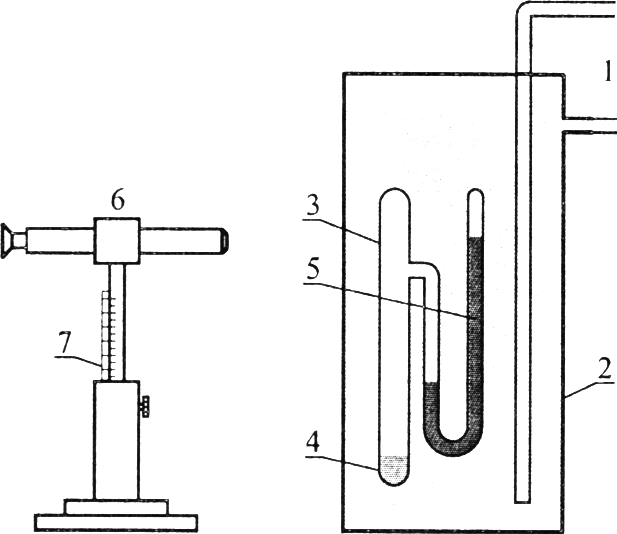
\includegraphics[width=0.95\textwidth]{apparatus}
			\captionof{figure}{Схема установки \label{apparatus}}
		\end{minipage}
		\hfill
		\begin{minipage}{0.35\textwidth}
			\textbf{Оборудование:} \\[.5ex]
			1 --- (к термостату) \\
			2 --- ёмкость с водой \\
			3 --- запаянная ёмкость \\
			4 --- исследуемая жидкость \\
			5 --- ртутный манометр \\
			6 --- отсчётный микроскоп \\
			7 --- штангенциркуль
		\end{minipage}
		\hfill~
		
		\bigskip
		\paragraph{Описание установки.} Заполненная водой ёмкость подключена
		к термостату. В неё погружена запаянная ёмкость с исследуемой жидкостью;
		над жидкостью находится только её насыщенный пар, давление которого
		определяется по манометру при помощи отсчётного микроскопа.
		Таким образом можно исследовать зависимость давления насыщенного пара
		исследуемой жидкости от температуры~$P(T)$, а затем определить~$L$
		с помощью~(\ref{eq:final}).
		
		Необходимо выдерживать скорость изменения
		температуры не слишком большой, поскольку в противном случае не будет успевать
		устанавливаться равновесие между теплообменной и исследуемой жидкостью, а также между
		исследуемой жидкостью и её парами. В целях контроля данные измерения производятся
		как при нагревании, так и при охлаждении жидкости.
		\newpage
		\section*{Выполнение работы}
		
		Работа состояла из двух частей. Сначала мы производили измерение температуры и показаний манометра при возрастании, а затем при убывании температуры (табл. 1, 2). Подсчеты было предложено произвести двумя способами: используя график $P(T)$(рис. 2) или используя график $\ln P (1/T)$, где $P=\rho g \Delta x$\\
		
		\begin{table}[h]

			\centering
		\begin{tabular}{|c|c|c||c|c|c|}
			\hline 
			$t, ^{\circ}C$ & $x_1$, см  & $x_2$, см & $P$, Па & $\ln P$ & $1/T$, 1/K \\ 
			\hline 
			23& 3,1 & 7,2 & 5535 & 8,61 & 0,003378 \\ 
			\hline 
			24& 2,9 & 7,6 & 6345 & 8,75 & 003367 \\ 
			\hline 
			25& 2,72 & 7,69 & 6710 & 8,81 & 0,003356 \\ 
			\hline 
			26& 2,5 & 7,84 & 7209 & 8,88 & 0,003344  \\ 
			\hline 
			27& 2,44  & 7,88 & 7344 & 8,9 & 0,003333\\ 
			\hline 
			28& 2,32 &  8,16 & 7884 & 8,97 & 0,003322\\ 
			\hline 
			29& 2,09 & 8,23 & 8289 & 9,02 & 0,003311 \\ 
			\hline 
			30& 1,93 & 8,5 & 8869,5 & 9,09 & 0,0033 \\ 
			\hline 
			31& 1,73 & 8,73 & 9450 & 9,15 & 0,003289\\ 
			\hline 
			32& 1,52 & 8,85 & 9895 & 9,2 & 0,003279\\ 
			\hline 
			33& 1,34 & 9,14 & 10530 & 9,26 & 0,003268\\ 
			\hline 
			34& 0,96 & 9,4 & 11394 & 9,34 & 0,003257\\ 
			\hline 
			35& 0,82 &  9,63 & 11893 & 9,38 & 0,003247\\ 
			\hline 
			36& 0,6 & 9,85 & 12488 & 9,43 & 0,003236\\ 
			\hline 
			37& 0,29 &  10,04 & 13162 & 9,49 & 0,003226\\ 
			\hline 
			38&  1,76 &  12,02 & 13851 & 9,54 & 0,003215\\ 
			\hline 
			\hline 
			33& 0,52 & 9,39 & 11975 & 9,31 & 0,003268\\ 
			\hline 
			32& 1,42 & 8,97 & 10193 & 9,23 & 0,003279\\ 
			\hline 
			30,5& 1,62 & 8,6 & 9423 & 9,15 & 0,003295\\ 
			\hline 
			30& 1,84 & 8,58 & 9099 & 9,12 & 0,0033\\ 
			\hline 
			29& 1,98 & 8,36 & 8613 & 9,06 & 0,003311 \\ 
			\hline 
			28& 2,18 & 8,13 & 8032 & 8,99 & 0,003322 \\ 
			\hline 
			27& 2,43 & 7,96 & 7465 & 8,92 & 0,003333\\ 
			\hline 
			26& 2,6 & 7,82 & 7047 & 8,86 & 0,003344\\ 
			\hline 
			25& 2,7 & 7,65 & 6682 & 8,81 & 0,003356\\ 
			\hline 
			24&  2,85&  7,52 & 6304 & 8,75 & 0,003367\\ 
			\hline 
			23& 3,02 & 7,35 & 5845 & 8,67 & 0,003378\\ 
			\hline 
						
					\end{tabular} \caption{Показания манометра и данные для графиков}

				\end{table}
				
	\newpage
	Для определения погрешности в первом случае будем использовать формулу 
	\begin{equation*}
	\sigma_L = L\cdot \left( \left(\dfrac{\sigma_P}{P}\right)^2 + 3\left(\dfrac{\sigma_T}{T}\right)^2 + \left(\dfrac{\sigma_{y'}}{a_y}\right)^2\right)^{\frac{1}{2}}.
	\end{equation*}
	Во втором случае:
	\begin{equation*}
	\sigma_L = L\cdot \dfrac{\sigma_{y'}}{y'} 
	\end{equation*}	
			
	\begin{minipage}{0.6\textwidth}
		\begin{tikzpicture}
		
		\begin{axis}[ xlabel={$T, K$},ylabel={$P, \textit{Па}$}, ymin = 5400, ymax = 14000, xmin = 296.5, xmax = 311.5,  grid = both, minor tick num =3, legend style = {anchor =  north west}]
		\addplot [color=blue, only marks, mark =x, error bars/.cd,
		x dir=both, x explicit, y dir=both, y explicit] table[col sep = semicolon, y index = 4, x index = 0, x error index = 11, y error index= 12] {data.csv};
		\addplot [color=red, only marks, mark = x, error bars/.cd, x dir=both, x explicit, y dir=both, y explicit] table[col sep = semicolon, y index = 10, x index = 6, x error index = 11, y error index= 12] {data.csv};
		\addplot [domain= 296.5:311.5] [color=blue, dashed] {11.69*x^2 - 6557.3*x + 922511};
		\addplot [domain= 296.5:307] [color=red, dashed] {16.79*x^2 - 9597.8*x + 1375782.24};
		\legend{Возр., Убыв.};
		\end{axis}
		\end{tikzpicture}
		
		\centering\captionof{figure}{График зависимости давления насыщенного пара жидкости $P\ \textit{(Па)}$ от времени $T\ \textit{(К)}$}
	\end{minipage}
	\hspace{0.5cm}
	\begin{minipage}{0.35\textwidth}
		\centering
		$y = 11,69 x^2 - 6557,3 x +922511$\\
		$y' = 23,38 x - 6557,3$\\
		$\sigma_{y'} = 0,06x$\\
		\vspace{1cm}
		$y=16,79 x^2 - 9597,8 x + 1375782$\\
		$y'=32,58 x - 9597,8$\\
		$\sigma_{y'} = 0,06x$\\
	\end{minipage}
	\vspace{1cm}
	
	
	По уравнению касательной к графику P(T) и используя уравнение \ref{eq:final} получим следующие значения $L$.\\
	
	\begin{minipage}{0.45\textwidth}
		\centering
	\begin{tabular}{|c|c|}
		\hline 
		T, $^{\circ} C$ & L, Дж/моль \\ 
		\hline 
		23 & $47770\pm 140$ \\ 
		\hline 
		24 & $44660\pm 120$ \\ 
		\hline 
		25 & $45100\pm 120$ \\ 
		\hline 
		26 & $44600\pm 110$ \\ 
		\hline 
		27 & $46510\pm 120$ \\ 
		\hline 
		28 & $45850\pm 120$ \\ 
		\hline 
		29 & $46030\pm 110$ \\ 
		\hline 
		30 & $45320\pm 100$ \\ 
		\hline 
		31 & $44710\pm 100$ \\ 
		\hline 
		32 & $44810\pm 90$ \\ 
		\hline 
		33 & $44110\pm 90$ \\ 
		\hline 
		34 & $42640\pm 80$ \\ 
		\hline 
		35 & $42670\pm 80$ \\ 
		\hline 
		36 & $42390\pm 80$ \\ 
		\hline 
		37 & $41890\pm 80$ \\ 
		\hline 
		38 & $41430\pm 80$ \\ 
		\hline 
	\end{tabular}\\ 
	$\overline{L} = (44,4\pm 0,1)\ \textit{кДж/моль}$
	\captionof{table}{Результаты при увеличении температуры}
		\end{minipage}
\hspace{1cm}
\begin{minipage}{0.45\textwidth}
	\centering
	\begin{tabular}{|c|c|}
		\hline 
		T, $^{\circ} C$ & L, Дж/моль \\ 
		\hline 
		33 & $47620\pm 100$  \\ 
		\hline 
		32 & $48850\pm 110$ \\ 
		\hline 
		30,5 & $48230\pm 110$  \\ 
		\hline 
		30 &$48390\pm 120$\\
		\hline
		29 &$47820\pm 110$  \\ 
		\hline 
		28 &$47790\pm 120$  \\ 
		\hline 
		27 &$4710\pm 120$  \\ 
		\hline 
		26 &$46670\pm 120$ \\ 
		\hline 
		25 & $45180\pm 120$\\ 
		\hline 
		24 & $43660\pm 120$ \\ 
		\hline 
		23 & $ 42690\pm 120$\\ 
		\hline 
		\end{tabular}\\ 
			$\overline{L} = (46,77\pm 0,11)\ \textit{кДж/моль}$
			\captionof{table}{Результаты при уменьшении температуры}
\end{minipage}
\vspace{1cm}


Теперь посчитаем $L$ вторым способом.
\vspace{1cm}


\begin{minipage}{0.6\textwidth}
	\begin{tikzpicture}
	
	\begin{axis}[ xlabel={$1/T, 1/K$},ylabel={$\ln P$}, ymin = 8.6, ymax = 9.6, xmin = 0.0032, xmax = 0.0034, minor tick num = 3, grid = both]
	\addplot [color=red, only marks, mark =x,  error bars/.cd,
	x dir=both, x explicit, y dir=both, y explicit] table[col sep = semicolon, y index = 18, x index = 9, y error index = 20, x error index = 22] {data.csv};
	\addplot [color=blue, only marks, mark = x,  error bars/.cd,
	x dir=both, x explicit, y dir=both, y explicit] table[col sep = semicolon, y index = 5, x index = 3, y error index = 19, x error index = 21] {data.csv};
	\addplot [domain= 0.0032:0.0034][color=blue, dashed] {-5376.7*x + 26.835};
	\addplot [domain = 0.0032:0.0034][color=red, dashed] {-5670*x + 27.847};
	\legend{Возр., Убыв.};
	\end{axis}
	\end{tikzpicture}
	
	\centering\captionof{figure}{График зависимости давления насыщенного пара жидкости $ln\ P\ \textit{(Па)}$ от времени $T\ \textit{(К)}$}
\end{minipage}
\hspace{0.5cm}
\begin{minipage}{0.35\textwidth}
	\centering
	$y = -5376,7 x + 26,835$\\
	$y' = -5370$\\
	$\sigma_{y'} = 7$\\
	$L = 44,67\pm 0,06\ \textit{кДж/моль}$\\
	\vspace{1cm}
	$y= -5670x+27,847$\\
	$y'=-5670$\\
	$\sigma_{y'} = 7$\\
	$L = 47,11\pm 0,06\ \textit{кДж/моль}$
\end{minipage}
\section*{Вывод}
Сравнивая табличное значение теплоты испарения спирта (48 кДж/моль) и полученные в результате работы значения, можно сказать, что они близки, но тем не менее есть неточности. Возможно, это связано с неаккуратным выполнением работы. Также, вероятно, использовался другой спирт с немного другими характеристиками.
\end{document}	